% For help on subfiles see https://www.sharelatex.com/learn/Multi-file_LaTeX_projects
\documentclass[../main.tex]{subfile}

\begin{document}
		
		\paragraph{} CuckooDroid is an extension of Cuckoo Sandbox the Open Source software for automating analysis of suspicious files. CuckooDroid brigs to cuckoo the capabilities of execution and analysis of android application \cite{cuckoodroid_docs}. For more information about the cuckoo sandbox, readers are encouraged to visit the cuckoo sandbox website \cite{cuckoo_website}.
		
		\paragraph{} CuckooDroid can be downloaded from the CuckooDroid github repository \cite{cuckoodroid_github} by following the guidelines provided there. For more step-by-step installation guide, readers are encouraged to have a look at CuckooDroid documentation \cite{cuckoodroid_docs}. Because of changes in android emulator (goldfish) and android SDK the CuckooDroid documentation are not precisely accurate and some deviations are required from it in order to make the CuckooDroid work. By following the CuckooDroid documentation with a few changes discussed later in this chapter, it should be fairly easy for reader to configure his CuckooDroid setup. 

		
		\subsection{CuckooDroid architecture}
		\paragraph{} In this section we will describe the architecture of CuckooDroid. There are main two parts a "Host" and a "Guest". Below is an excerpt from the CuckooDroid documentation \cite{cuckoodroid_docs}:
		
		\say{This documentation refers to Host as the underlying operating systems on which you are running Cuckoo (generally being a GNU/Linux distribution) and to Guest as the Windows virtual machine used to run the isolated analysis.}
		
		\paragraph{} We will be configuring CuckooDroid with Android Emulator (Goldfish) and figure \ref{fig:cuckoodroid_avd_arch} shows the architecture CuckooDroid with Android Emulator. As it can be seen in the figure \ref{fig:cuckoodroid_avd_arch} that there are two main parts, Cuckoo Sandbox and Android Emulator.
		
		\begin{figure}
			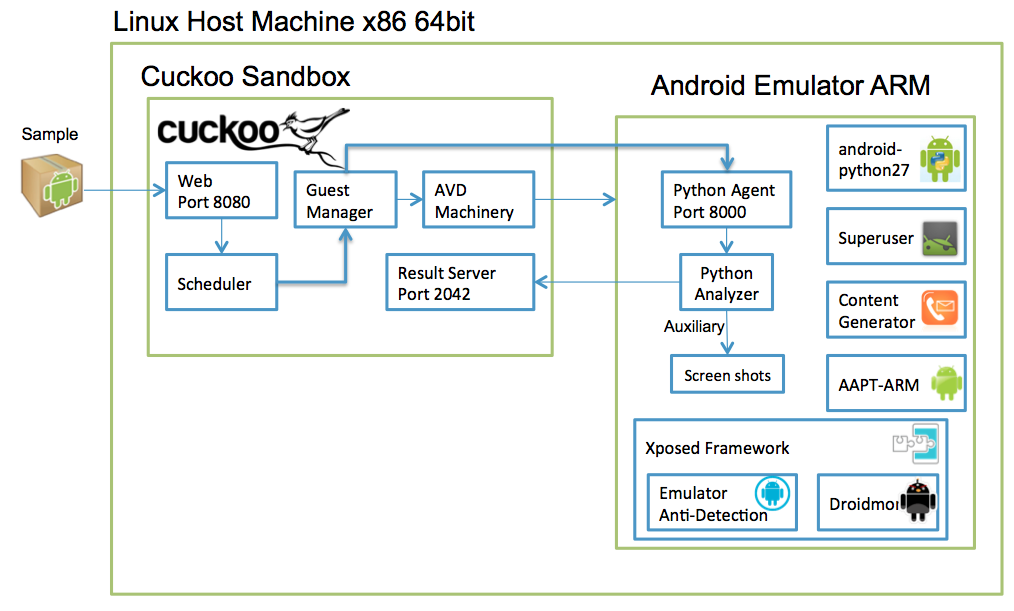
\includegraphics[width=\textwidth]{android_avd_arch.png}
			\caption{CuckooDroid architecture with AVD}
			\label{fig:cuckoodroid_avd_arch}
		\end{figure}
		
		\paragraph{} Cuckoo Sandbox is responsible for managing the android emulator and generating report at the end of analysis. Android Emulator executes the application, gather some information from it and reports it back to Cuckoo Sandbox. Below is the description of some of the main parts shown in figure \ref{fig:cuckoodroid_avd_arch}
		\begin{itemize}
			\item \textbf{Python Agent} Executed on AVD and is responsible for receiving APK file, Analysis code, configuration and executing analysis. It also provides constant status updates to Host.
			\item \textbf{Python Analyzer} Android analyzer component that is sent to the guest machine at the beginning of the analysis. This is the main part that executes application, send dropped files back to host, send screenshots back to host, interact with the application if required. It is also responsible for ending the analysis and sending back some log files back to host. It has modular structure and new modules can be added very easily.
			\item \textbf{Xposed Framework} A framework for modules that can change the behavior of the system and apps without affecting any APKs. The version in use only work up to Android 4.1.2 (API 16). In CuckooDroid two modules are used with this Framework:
			\begin{enumerate}

				\item \textbf{Droidmon:} Dalvik  API Call monitoring module, it hooks up API calls and prints it into logcat, anaylsis code takes it form logcat and store it in a log file which is sent back to host at the end of anaylsis.
				\item \textbf{Emulator Anti-Detection:} Implements some know Emulator Anti-detection techniques (For more details on this topic see Chapter \ref{sec:Chp4})
			\end{enumerate}
		\end{itemize}
		
		\subsection{CuckooDroid required patching}
		\todo[inline]{Fixing cuckoodroid}
		\subsection{Android emulator and its rooting}
		\todo[inline]{Persistent root problem}
		\subsection{Upgrading to higher versions of Android}
		\todo[inline]{Latest android}
		\subsubsection{NDK hello world, python termux}
		\todo[inline]{python compilation workaround, termux}
		\subsection{Future work}
		\todo[inline]{Slow android emulator}
		\todo[inline]{Emulator anti detection}

\end{document}